\documentclass{article}
\usepackage[T1]{fontenc}
\usepackage[utf8]{inputenc}
\usepackage[english]{babel}
\usepackage[margin=3cm]{geometry}
\usepackage{amsmath, amssymb}
\usepackage{amsfonts}
\usepackage{dsfont}
\usepackage{float}
\usepackage{graphicx}
\usepackage{wrapfig}
\usepackage{mathtools}
\usepackage{bbm}
\usepackage{amsthm}
\usepackage{ifthen}
\usepackage{graphicx}
\usepackage{hyperref}
\usepackage[ruled,vlined]{algorithm2e}
\usepackage{xcolor}
\usepackage{mathtools}
\usepackage{empheq}
\usepackage{subfig}
\usepackage{tikz}
%\usepackage{hyperref}
%\usetikzlibrary{shapes.multipart}
%\usepackage[demo]{graphicx}
%\DeclarePairedDelimiter{\ceil}{\lceil}{\rceil}

\newtheorem{theorem}{Theorem}[section]
\newtheorem{prop}[theorem]{Proposition}
%\theoremstyle{definition}
\newtheorem{definition}[theorem]{Definition}
\newtheorem{remark}{Remark}[section]
\newtheorem{lemma}[theorem]{Lemma}
\newtheorem{Cl}{Claim}[section]

\newcommand{\ca}[1]{\mathcal{#1}}
\newcommand{\bb}[1]{\mathbb{#1}}
\newcommand{\p}{\mathbb{P}}
\newcommand{\evento}[1]{\left\{ \textit{``#1''} \right\}}
\newcommand{\comillas}[1]{``#1''}
\newcommand{\set}[1]{\left\{#1\right\}}
\newcommand{\parent}[1]{\left(#1\right)}
\newcommand{\parentCuad}[1]{\left[#1\right]}
\newcommand{\borel}{\ca{B}(\bb{R}^d)}
\newcommand{\Rd}{\bb{R}^d}
\newcommand{\R}{\bb{R}}
\newcommand{\infNorm}[1]{||#1||_\infty}
\newcommand{\condExp}[2]{\bb{E}(#1|#2)}
\newcommand{\ind}[1]{\mathbbm{1}_{#1}}
\newcommand{\esp}[1]{\bb{E}\barras{#1}}
\newcommand{\indep}{\rotatebox[origin=c]{90}{$\models$}}
\newcommand{\X}{$(X_t)_t\ $}
\newcommand{\pe}{$(\Omega, \ca{F}, \p)\ $}
\newcommand{\vc}[1]{\langle #1 \rangle}
\newcommand{\gb}[1]{\overline{\widehat{#1}}}
\newcommand{\barras}[1]{\left| #1 \right|}
\newcommand{\integral}{\int_{t_i}^{t_{i+1}}}
\newcommand{\ug}[1]{\widehat{\ca{U}}_{#1}}
\newcommand{\vg}[1]{\widehat{\ca{V}}_{#1}}
\newcommand{\norm}[1]{\left\lVert#1\right\rVert}
\newcommand{\xscheme}[1]{X_{t_{#1}}^{\pi}}
\newcommand{\prom}[1]{\langle #1 \rangle}
\newcommand*\widefbox[1]{\fbox{\hspace{2em}#1\hspace{2em}}}

\begin{document}
\section{Introducción}

\section{Objetivos y Metodología}
    Se propone una investigación enfocada en estudiar y evaluar la aplicación del \comillas{Procesamiento de lenguaje natural}
    o NLP por su sigla en inglés para construir un índice económico.

\section{Desarrollo}
    Lo primero es definir y entender para que sirve un índice económico, desde ahora simplemente \comillas{índice}. Este se puede definir como un indicador estadístico asociado a un conjunto de instrumentos financieros, en este trabajo sólo se consideran bonos y acciones, matemáticamente se puede definir como una serie de tiempo $(X_t)_{t=1}^{N}$ indexada por día. También, se denota como índice al conjunto de instrumentos seleccionados para su construcción. El cálculo del índice se puede hacer de variadas formas dependiendo de la naturaleza de los instrumentos que lo componen, generalmente se hace uso de un promedio ponderado de los precios de los instrumentos en el índice. Por ejemplo, suponiendo un conjunto $I$ de
    instrumentos financieros, claramente finito, podemos computar el valor de nuestro índice al día $t$ como:
    
    \begin{align*}
    	X_t = \frac{1}{|I|}\sum_{i \in I} P(i)_t.
    \end{align*}
    
   	Donde $P(i)$ corresponde a la serie de precios del instrumento $i$. Este tipo de índices se usan como indicadores de que tan fructífera ha sido la economía, una subida en este valor se puede entender como un alza en los precios y por lo tanto, un \comillas{alza del sector económico} y viceversa. Uno de los índices más importantes es el \textbf{S\&}\textbf{P 500} de Estados Unidos, país que al ser potencia mundial influye en la economía del resto del mundo, este índice se compone de $500$ acciones las cuales cotizan en la primera y segunda bolsa de valores más importantes de EE.UU, la de Nueva York o NYSE (New York Stock Exchange) y NASDAQ (National Association of Securities Dealers Automated Quotation), también ubicada en Nueva York, correspondientemente. En el caso de Chile, existe el \textbf{IPSA} o Índice de Precio Selectivo de Acciones, este agrupa las $30$ acciones con mayor presencia bursátil en el mercado y es reajustado cada año haciendo entrar y salir acciones.
    


\subsection{Replicación IPSA}
   	La primera parte del trabajo realizado se basó en replicar los valores del \textbf{IPSA} con los datos disponibles. La información entregada por \textbf{LVA} corresponde a los datos de transacciones diarias en la Bolsa de Santiago, agrupados por mes en distintos archivos. 
    Estos datos se ven como se muestra en la Figura \ref{fig:trans}.
   	\begin{figure}[H]
   		\centering
   		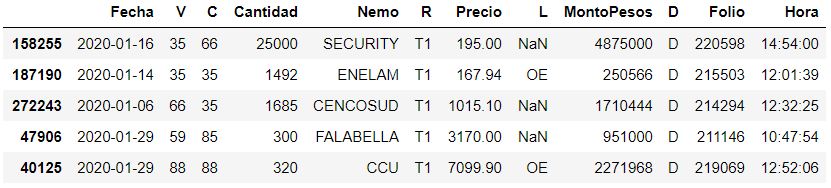
\includegraphics[scale=.5]{imgs/transacciones_RV_data.png}
   		\caption{Muestra de tamaño $5$ de datos disponibles para replicación del IPSA, enero $2020$.}
   		\label{fig:trans}
   	\end{figure}
    
   	La columna \textit{Folio} identifica unívocamente a cada transacción, \textit{Precio} indica el precio al cual se transó,  \textit{Cantidad} la cantidad de acciones transadas, \textit{MontoPesos} corresponde a la multiplicación de las dos anteriores y \textit{Nemo} es la etiqueta que se le da a la acción en la bolsa, generalmente corresponde al nombre de la empresa que emite la acción. Algunos de estos Nemos son: BSANTANDER, FALABELLA y ENELCHILE, por ejemplo. El resto de las columnas no será relevante para este estudio.\\
   	
   	\begin{remark}
   		La mayoría de los datos financieros no incluyen fechas que correspondan a fines de semana o festivos. Esto se debe a que las instituciones que generan estos datos no trabajan en tales días.
   	\end{remark}
   	
   	\begin{remark}
   		El análisis no estuvo exento de datos dañados. Las primeras aproximaciones al IPSA se caracterizaban por \textit{peaks} severamente pronunciados o fechas en las cuales los valores obtenidos simplemente no tenían sentido. Estos problemas se deben a que en el caso de no tener el dato, este era reemplazado por un $-1000$ y además, existe un rango de fechas, específicamente en el mes de marzo del $2020$, en las cuales los datos no fueron llenados correctamente (ver Figura \ref{fig:danados}). Esta situación fue confirmada por el supervisor y se decide simplemente eliminar estas filas dañadas. 
   		
   		\begin{figure}[H]
   			\centering
   			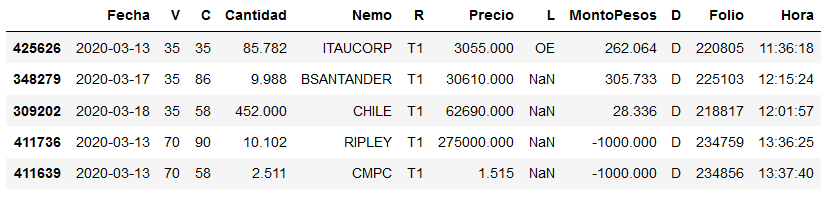
\includegraphics[scale=.5]{imgs/muestra_danada.png}
   			\caption{Muestra de datos dañados.}
   			\label{fig:danados}
   		\end{figure}
   		
   	\end{remark}
   	
   	Lo primero que se necesita es estimar el precio de una acción en un día cualquiera. Para esto nos fijamos en una acción (o Nemo) y fecha cualquiera, a modo de ejemplo tomamos \textbf{CCU} y el $15$ de abril del $2020$. Para este par existen $456$ transacciones (ver Figura \ref{fig:ccu_abril}).   
   	\begin{figure}[H]
   		\centering
   		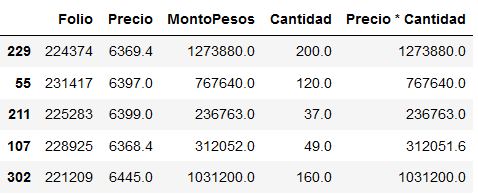
\includegraphics[scale=.5]{imgs/ccu_abril.png}
   		\caption{Muestra de tamaño $5$ de las transacciones asociadas a \textbf{CCU} el 15 de abril del $2020$.}
   		\label{fig:ccu_abril}
   	\end{figure}
   	Se decide calcular el precio del día como un promedio de \textit{Precios} ponderando por \textit{MontoPesos}.
    \begin{align*}
        X_t = \sum_{i\in I} P(i)_t w(i)
    \end{align*}


    donde $w(i)$ es un peso que representa la capitalización de cada instrumento y es invariante 
    con respecto a $t$.

	\begin{figure}[H]
		\centering
		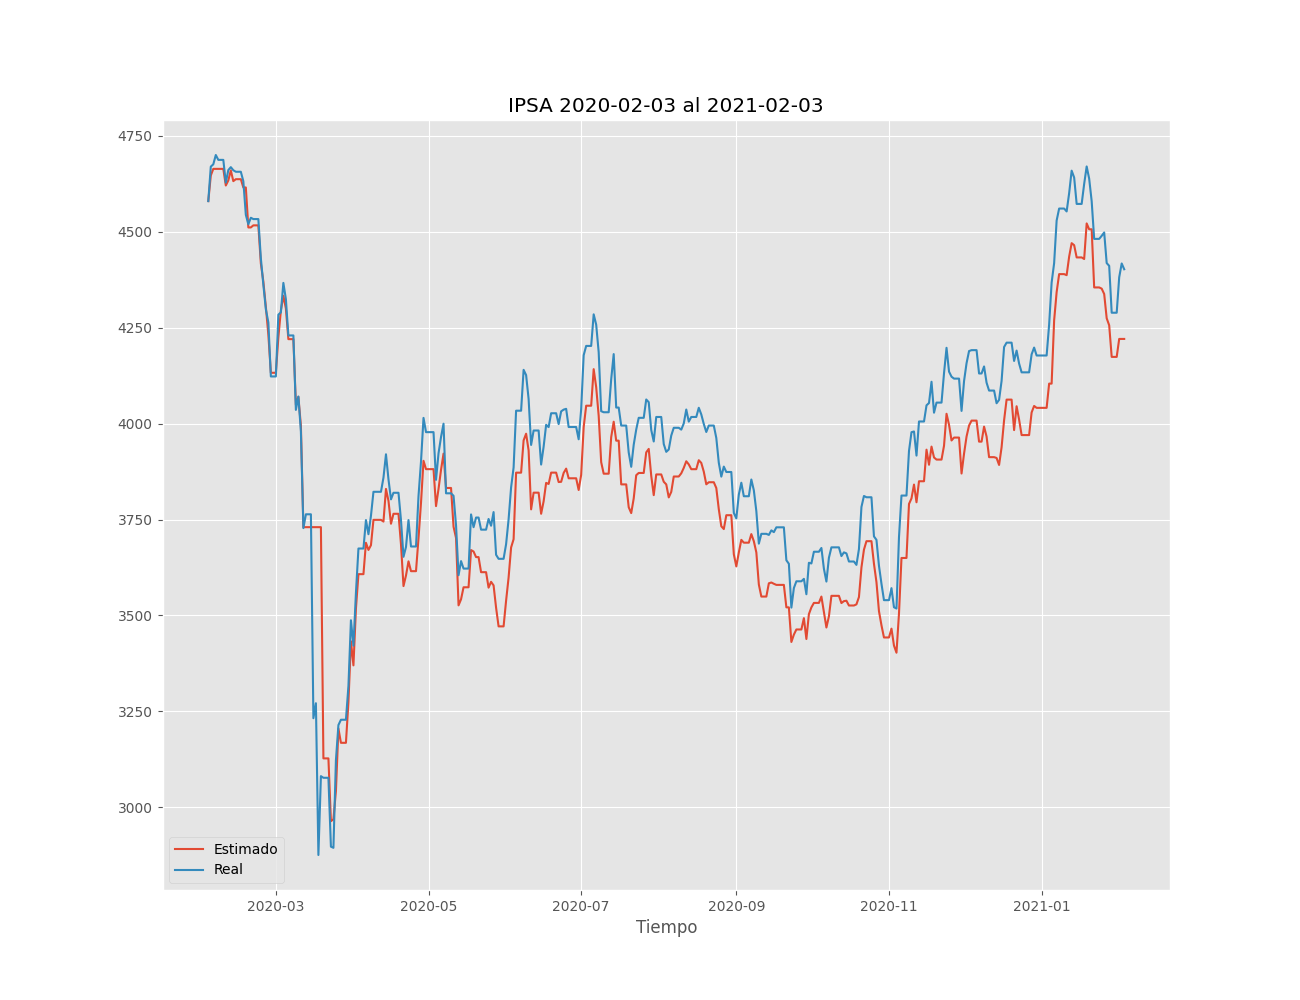
\includegraphics[scale=.25]{imgs/ipsa_replication.png}
		\caption{Replicación del ipsa.}
		\label{fig:ipsa_replication}
	\end{figure}



\section{Punto de que hablar}
    \begin{enumerate}
        \item Calculo de índices: IPSA. Explicar el cálculo del índice y por qué se calcula este tipo de indicadores.
        \item Análisis de sentimientos con twitter: Hablar de la cantidad de data por nemo y poner gráfico de barras.
        \item Hablar de la decisión de dejar retweets porque representan el mismo comentarios pero de otra persona.
        \item Comentar que hay tweets en otros idiomas y por lo tanto se hizo necesario trabajar con APIs de idioma.
        \item Series de tiempo en economía.
        \item Correlación entre dos variables. 
        \item Test de correlación.
        \item Explicar el cálculo del sentimiento saturado, shifted y todo el preproceso que se le hace a los valores pos, neu y neg para transformarlos en un número representativo del sentimiento de cada tweet
        \item Explicar que el sentimiento del día asociado a un instrumento se calcula como un promedio de los score de tweets diarios.
        \item Explicar que se busca parámetros que maximicen la correlación entre las variables adecuadas: \textbf{retorno} del sentimiento, sentimiento promedio en el periodo \textbf{sent days}, promedio de los retornos diarios, etc contra el retorno del precio de la acción o menos la tasa de interés para el caso de bonos.
        \item Mostrar los gráficos del índice obtenido y los nemos que participan del índice.
    \end{enumerate}


\end{document}
